%%%%%%%%%% Related work
\nop{\tc{
	I will discuss what other people have done regarding
	the problems in Introduction: 
	what formalisms of preferences have been
	introduced, what solutions have been proposed to solve
	these problems.
}}

In this section I will present work related to my thesis research.
I will first review some of the preference
systems studied in the literature that are designed to represent
qualitative preferences over combinatorial domains. 
I will then introduce concepts
from social choice theory underlying methods to
combine individual preferences to reach a common decision.

\section{Preferences Modeling and Reasoning \label{sec:pref_reasoning}}
Researchers have proposed several languages to model preferences.
I will now discuss those of them that are closely related
to my work.
These languages include graphical formalisms:
\tit{Conditional Preference Networks} (CP-nets) and
\tit{Lexicographic Preference Trees} (LP-trees);
and logical formalisms:
\tit{Possibilistic Logic} and
\tit{Answer Set Optimization} (ASO).
They are developed to provide concise and intuitive
presentations of preferential information for objects from
combinatorial domains.

For all systems, I will focus on two aspects:
the language in which preferences are specified,
and complexity of and algorithms for
problems about the model.
The most fundamental of these problems are introduced
in the following definitions.

\nop{{\bf [THESE DEFINITIONS ARE AT A WRONG PLACE.]}}
\begin{definition}
\label{def:con}
  $\cL$-CONSISTENCE: given an instance $\cC$ of a preference
	formalism $\cL$, decide whether $\cC$ is consistent, that is,
  whether there exists a total order of outcomes that agrees with every
	preference statement in $\cC$.
\end{definition}

\begin{definition}
\label{def:dom}
  $\cL$-DOMINANCE: given an instance $\cC$ of a preference
	formalism $\cL$ and its two distinct outcomes
  $o_1$ and $o_2$, decide whether $o_1 \succ_\cL o_2$, that is,
  whether $o_1$ is strictly preferred to $o_2$ in $\cC$.
\end{definition}

\begin{definition}
\label{def:opt1}
  $\cL$-OPTIMALITY-\rom{1}: given an instance $\cC$ of a preference
	formalism $\cL$,
  decide whether $\cC$ has an optimal outcome.
\end{definition}

\begin{definition}
\label{def:opt2}
  $\cL$-OPTIMALITY-\rom{2}: given an instance $\cC$ of a preference
	formalism $\cL$ and an outcome $o$ of $\cC$,
  decide whether $o$ is an optimal outcome.
\end{definition}

\begin{definition}
\label{def:opt3}
  $\cL$-OPTIMALITY-\rom{3}: given an instance $\cC$ of a preference
	formalism $\cL$ and some property $\Phi$ expressed as a Boolean formula 
	over the alphabet of $\cC$,
  decide whether there is an optimal outcome $o$ that satisfies $\Phi$.
\end{definition}

\subsection{Conditional Preference Networks}
\noindent{\textbf{The Language.}}
Conditional Preference Networks (CP-nets) define preferential relations between outcomes
based on the \tit{ceteris paribus}
semantics \cite{bbdh03}.
\textit{Ceteris paribus} is latin for ``everything else being equal."

Let $\bV$ be a set of binary attributes\footnote{
	Attributes in CP-nets can be multi-valued. However,
	as my research mostly deals with preference models over
	binary attributes, it suffices to discuss CP-nets
	in such a setting.
}
, we denote by $\Asst(\bV)$ the set of
all truth assignments to the attributes in $\bV$.
For each attribute $X_i \in \bV$, $\Pa(X_i)$ denotes the \tit{parent} attributes of
$X_i$, such that preferences over the domain of $X_i$ depend upon how
$\Pa(X_i)$ are evaluated.
%\begin{definition}
%\label{def:pi}
%	A set of attributes $\bX$ is \tit{preferentially independent}
%	of $\bY=\bV-\bX$ if $\forall \bx_1,\bx_2 \in \Asst(\bX)$ and
%	$\forall \by_1,\by_2 \in \Asst(\bY)$,
%	\begin{center}
%		$\bx_1\by_1 \succeq \bx_2\by_1 \; \itiff \; \bx_1\by_2 \succeq \bx_2\by_2$.
%	\end{center}
%\end{definition}
%
%\begin{definition}
%\label{def:cpi}
%	Let $\bX$, $\bY$ and $\bZ$ be nonempty sets such that
%	$\bX \cup \bY \cup \bZ = \bV$.
%	$\bX$ is conditionally preferentially independent
%	of $\bY$ given an assignment $\bz$ to $\bZ$ 
%	if $\forall \bx_1,\bx_2 \in \Asst(\bX)$ and
%	$\forall \by_1,\by_2 \in \Asst(\bY)$,
%	\begin{center}
%		$\bx_1\by_1\bz \succeq \bx_2\by_1\bz \; \itiff \; \bx_1\by_2\bz \succeq \bx_2\by_2\bz$.
%	\end{center}
%\end{definition}
%
%\begin{definition}
%	For each attribute $X_i$, $\Pa(X_i)$ denotes its parent attributes such that,
%	given an assignment to $\Pa(X_i)$, $X_i$ is conditionally preferentially independent
%	of $\bV-(\Pa(X_i) \cup \{X_i\})$.
%\end{definition}

\begin{definition}
\label{def:cpn}
	Let $\bV$ be a set of binary attributes $\bV=\{X_1,\ldots,X_n\}$.
	A CP-net over $\bV$ is a tuple ($G$,$T$), where
	\begin{enumerate} \itemsep -4pt
		\item $G$ is a directed graph ($V,E$) specifying
					dependencies among attributes,
					where for every $X_i \in V$ we have
					$\Pa(X_i)=\{X_j:(X_j,X_i) \in E\}$,
		\item $T$ is a collection of 
					conditional preference tables (CPTs) for
					all attributes.  A $\CPT(X_i)$ consists of preference
					statements of the form
					\begin{center}
						$\bu : \succ^i_{\bu}$,
					\end{center}
					where $\bu \in \Asst(\Pa(X_i))$ and $\succ^i_{\bu}$
					is a total order over $\Dom(X_i)$ given $u$.
	\end{enumerate}
\end{definition}

\nop{\mc{Need an example of CP-net here.}}
We say that a CP-net $N=(G,T)$ is \tit{acyclic} if
$G$ is acyclic; \tit{cyclic}, otherwise.
To illustrate, let us consider the domain of cars.
For simplicity, we take three binary attributes
\tit{Price}, \tit{Safety}, and \tit{Capacity}.
Attribute \tit{Capacity} ($C$) has two values \tit{high} ($c$) 
and \tit{low} ($\bar{c}$).
Attribute \tit{Price} ($P$) has two values \tit{high} ($p$) 
and \tit{low} ($\bar{p}$).
Attribute \tit{Safety} ($S$) has two values \tit{high} ($s$) 
and \tit{low} ($\bar{s}$).
An example CP-net $N=(G,T)$ over binary attributes $\bV=\{C,P,S\}$
is shown in \figref{CPN_depend}.
The directed graph $G$, also called the \tit{dependency graph}, expresses
dependencies among attributes.  An arrow in the dependency graph points
to a child attribute from a parent attribute. Thus, we see that,
the preferences on \tit{Price} (\tit{Safety}) depend upon the assignment made
to \tit{Capacity} (\tit{Price}, respectively).

\nop{\noindent{\textbf{The Model.}}}
To decide if outcome $o_1$ is preferred to outcome $o_2$ in a CP-net $N$,
one needs to show that $o_2$ can be improved, ceteris paribus, 
according to the preference statements in $N$ to reach $o_1$.

\begin{definition}
	Let $N$ be a CP-net over $\bV$, $X_i \in \bV$, $\bU = \Pa(X_i)$,
	and $\bY=\bV-(\bU \cup \{X_i\})$.
	Let $\bu x_i \by$ be an outcome, where $x_i\in \Dom(X_i)$,
	$\bu \in \Asst(\bU)$, and $\by \in \Asst(\bY)$.
	An \tit{improving flip} of $\bu x_i \by$ wrt $X_i$ is an
	outcome $\bu x_i' \by$ such that $x_i' \succ^i_{\bu} x_i$.
	A \tit{sequence of improving flips} wrt $N$ is a sequence of
	outcomes $o_1,\ldots,o_j$ such that, for every $k<j$,
	$o_{k+1}$ is an improving flip of $o_k$ wrt some attribute in $\bV$.
	We say that outcome $o_1$ is preferred to outcome $o_2$ in $N$,
	denoted by $o_1 \succ_N o_2$, if there exists a sequence of
	improving flips from $o_2$ to $o_1$.
\end{definition}

In a CP-net $N$, we say that outcome $o$ is \tit{optimal} if
there does not exist another outcome $o'$ such that
$o' \succ_N o$.

%\begin{definition}
%	Let $N$ be a CP-net over $\bV$, $X_i \in \bV$, and $\bU = \Pa(X_i)$.
%	Given an assignment $\bu$ to $\bU$,
%	a total order $\succ$ over $\Asst(\bV)$ \textit{satisfies}
%	$\succ^i_{\bu}$ if for all $\by \in \Asst(\bY)$ and all
%	$x,x' \in \Dom(X_i)$, $\bu \it{x} \by \succ \bu \it{x'} \by$ whenever
%	$x \succ^i_{\bu} x'$.
%	$\succ$ \textit{satisfies}
%	$\CPT(X_i)$ if it satisfies $\succ^i_{\bu}$ for each
%	$\bu \in \Asst(\bU)$.
%	$\succ$ \textit{satisfies}
%	the CP-net $N$ if it satisfies $\CPT(X_i)$ for every $X_i$.
%	A CP-net $N$ is \textit{consistent} $\itiff$ there exists a total order
%	$\succ$ that satisfies $N$.
%\end{definition}

Consider the CP-net $N$ in \figref{CPN}.
It induces a partial order shown in \figref{CPN_pref},
where each arrow represents an improving flip between two outcomes.
We see that $c\bar{p}\bar{s} \succ_N \bar{c}ps$
because of the improving flipping sequence --
$c\bar{p}\bar{s},\bar{c}\bar{p}\bar{s},\bar{c}\bar{p}s,\bar{c}ps$.
Outcome $cps$ is optimal because no other outcome is
better.
We note that there is no flipping sequence between
$c\bar{p}s$ and $\bar{c}\bar{p}\bar{s}$.
In such case, we say that the two outcomes are \tit{incomparable}.
This CP-net is consistent because there exists a total order
of outcomes that agrees with the preference graph \figref{CPN_pref}.
There are in fact two such total orders:

\begin{center}
	$cps \succ cp\bar{s} \succ c\bar{p}\bar{s} 
		\succ \bm{c\bar{p}s} \succ \bm{\bar{c}\bar{p}\bar{s}} 
		\succ \bar{c}\bar{p}s \succ \bar{c}ps \succ \bar{c}p\bar{s}$,\\
	$cps \succ cp\bar{s} \succ c\bar{p}\bar{s} 
		\succ \bm{\bar{c}\bar{p}\bar{s}} \succ \bm{c\bar{p}s}
		\succ \bar{c}\bar{p}s \succ \bar{c}ps \succ \bar{c}p\bar{s}$.
\end{center}

%\begin{figure}[h!]
%  \centering
%  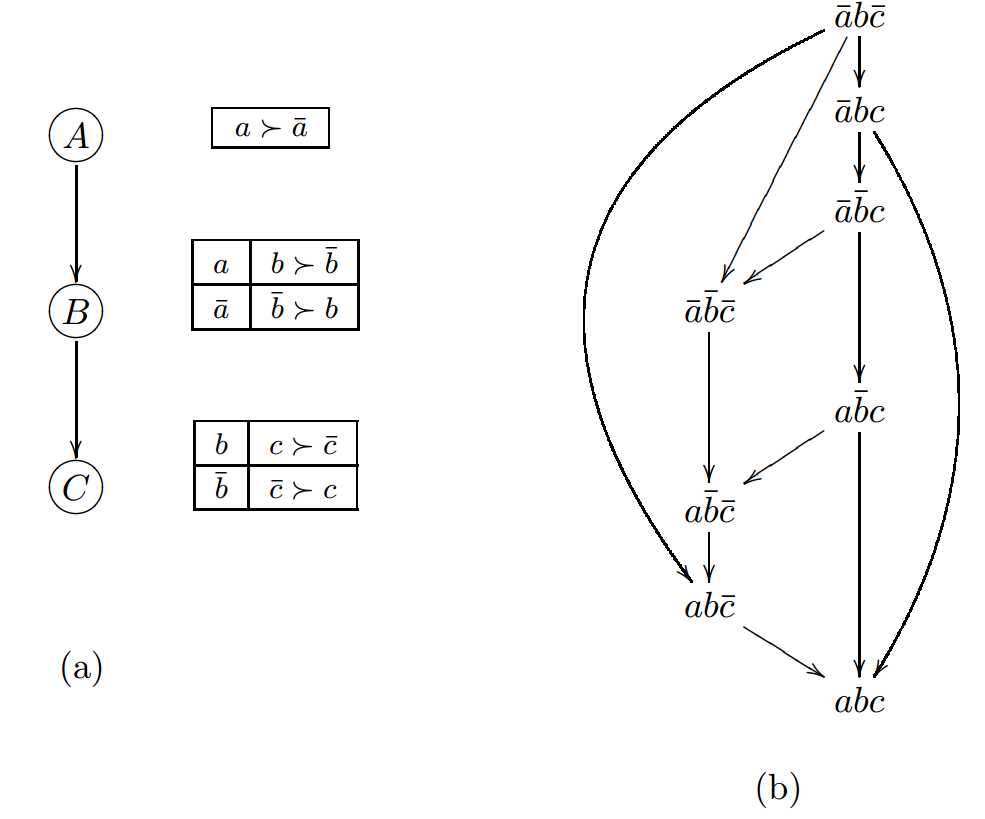
\includegraphics[width=0.7\textwidth]{img/acpn.png}
%  \caption{Acyclic CP-net \label{fig:cp_net}}
%\end{figure}

\begin{figure}[!ht]
	\centering
  \begin{subfigure}[b]{0.45\textwidth}
		\centering
	  \begin{tikzpicture}[->,>=stealth',
	    level/.style={sibling distance=2cm/#1, level distance=40pt}]
	    \node [main node] (1){$C$}
	      child {node [main node] (2) {$P$}
	      	child {node [main node] (3) {$S$} {}
							child {node [rectangle,draw] (4) at (1.7,4.2) {$c>\bar{c}$} edge from parent[draw=none]}
							child {node [rectangle split, rectangle split parts=2,draw] (5) at (1.35,2.8)
								{$c:p>\bar{p}$ \nodepart{second} $\bar{c}:\bar{p}>p$} edge from parent[draw=none]}
							child {node [rectangle split, rectangle split parts=2,draw] (6) at (0.7,1.4) 
								{$p:s>\bar{s}$ \nodepart{second} $\bar{p}:\bar{s}>s$} edge from parent[draw=none]}
					}
	      };
	  \end{tikzpicture}
		\caption{Dependency graph and CPT's\label{fig:CPN_depend}}
	\end{subfigure}%
  \begin{subfigure}[b]{0.45\textwidth}
		\centering
		  \begin{tikzpicture}[->,>=stealth',node distance=1cm,main node/.style={circle,draw,font=\small}]
		    \node[rectangle,inner sep=0pt] (1)                                         {$\bar{c}p\bar{s}$};
				\node[rectangle,inner sep=0pt] (2) [below of=1]                            {$\bar{c}ps$};
				\node[rectangle,inner sep=0pt] (3) [below of=2]                            {$\bar{c}\bar{p}s$};
				\node[rectangle,inner sep=0pt] (4) [left of =3,xshift=-1cm,yshift=-0.5cm]  {$\bar{c}\bar{p}\bar{s}$};
				\node[rectangle,inner sep=0pt] (5) [below of=3]                            {$c\bar{p}s$};
				\node[rectangle,inner sep=0pt] (6) [left of=5,xshift=-1cm,yshift=-0.5cm]   {$c\bar{p}\bar{s}$};
				\node[rectangle,inner sep=0pt] (7) [below of=6]                            {$cp\bar{s}$};
				\node[rectangle,inner sep=0pt] (8) [below of=5,yshift=-1cm]                {$cps$};
		
		    \path[every node/.style={font=\sffamily\small}]
		      (1) edge (2)
		      (1) edge (4)
		      (1) edge [bend right=70] (7)
		      (2) edge (3)
		      (2) edge [bend left=40] (8)
		      (3) edge (4)
		      (3) edge (5)
		      (4) edge (6)
		      (5) edge (6)
		      (5) edge (8)
		      (6) edge (7)
		      (7) edge (8);
		  \end{tikzpicture}
		\caption{Preference graph\label{fig:CPN_pref}}
	\end{subfigure}
  \caption{Acyclic CP-net}
  \label{fig:CPN}
\end{figure}

%Answering the CP-CONSISTENCE problem depends upon whether
%its dependency graph are acyclic and how preference rules
%in CPTs are specified.
%Researchers in AI have been working on this problem
%and many results can be found in the literature.



\noindent{\textbf{Problems and Complexity.}}
Boutilier, Brafman, Domshlak, Hoos and Poole \cite{bbdh03} 
have proved that every acyclic CP-net
is consistent, whereas Goldsmith, Lang, Truszczynski and Wilson \cite{Goldsmith}
have shown that the CPN-CONSISTENCE problem is PSPACE-complete in general.

For the CPN-DOMINANCE problem, its complexity depends on the structure
of the dependency graph.
The CPN-DOMINANCE problem can be solved by
a polynomial time algorithm for binary-valued tree-structured
CP-nets, and that the problem is NP-complete for binary-valued
CP-nets with specially structured dependency graphs 
(e.g., max-$\delta$-connected dependency graphs) \cite{bbdh03}.
However, it is NP-hard for general binary-valued acyclic 
CP-nets \cite{bbdh03}.
Furthermore, in the most general case when the dependency graph
could be cyclic, this problem is PSPACE-complete even
if the CP-nets are consistent \cite{Goldsmith}.

For acyclic CP-nets, the optimality problems (i.e.,
CPN-OPTIMALITY-\rom{1}, CPN-OPTIMALITY-\rom{2}, and
CPN-OPTIMALITY-\rom{3}) are easy \cite{bbdh03}.



\subsection{Lexicographic Preference Trees \label{sec:LPT}}
The language of lexicographic preference trees \cite{booth:learningLP} 
uses trees to model preferences. It is motivated by lexicographic
orderings \cite{Kaci:Pref} and lexicographic preferences \cite{10.2307/2296854}.
This formalism and its variants are the primary focus on my research.

\noindent{\textbf{The Language.}}
\tit{A lexicographic preference tree} (\emph{LP-tree}) $T$ over a set $\cI$ 
of $p$ binary attributes $X_1,\ldots,X_p$ is a labeled \emph{binary tree}. Each
node $t$ in $T$ is labeled by an attribute from $\cI$, denoted by 
$\mathit{Iss}(t)$, and with \emph{preference information} of the form
$a>b$ or $b>a$ indicating which of the two values $a$ and $b$  comprising
the domain of $\Iss(t)$ is preferred (in general the preference may depend
on the values of attributes labeling the ancestor nodes). We require that 
each attribute appears exactly once on each path from the root to a leaf. 

Intuitively, the attribute labeling the root of an LP-tree is of highest 
importance. Alternatives with the preferred value of that attribute
are preferred over outcomes with the non-preferred one. The two
subtrees refine that ordering. The left subtree determines the ranking
of the preferred ``upper half'' and the right subtree determines the 
ranking of the non-preferred ``lower half.'' In each case, the same 
principle is used, with the root attribute being the most important one. 
\nop{The attribute labeling the root of a subtree is the
most important among those appearing in the subtree, and the outcomes
the subtree represents are split into the preferred and non-preferred 
halves based on their value and on the preference information at the node.}
We note that the attributes labeling the roots of the 
subtrees need not be the same (the relative importance of attributes may 
depend on values for the attributes labeling the nodes on the path to the root).

The precise semantics of an LP-tree $T$ captures this intuition. Given 
an outcome $x_1x_2\ldots x_p$, we find its preference ranking in 
$T$ by traversing the tree from the root to a leaf. When at node $t$ 
labeled with the attribute $X_i$, we follow down to the left subtree if
$x_i$ is preferred according to the preference information at node
$t$. Otherwise, we follow down to the right subtree. 

It is convenient to imagine the existence of yet another level of nodes 
in the tree, not represented explicitly, with each node in the lowest 
level ``splitting'' into two of these
implicit nodes, each representing an outcome. Descending the tree 
given an outcome in the way described above takes us to an (implicit) 
node that represents precisely that outcome's rank.
The more to the left the node representing the outcome, the more 
preferred it is, with the one in the leftmost (implicit) node being the 
most desirable one as left links always correspond to preferred values.

To illustrate these notions, let us consider an example LP-tree
over the car domain, given by the three binary attributes 
\tit{Capacity}, \tit{Price}, and \tit{Safety},
described as earlier.
Our agent prefers cars with high capacity to cars with low capacity,
and this preference on \tit{Capacity} is the most important one.
Then, for high-capacity cars, the next most important attribute is
\tit{Safety} and she prefers cars with high security level,
and the least important attribute is \tit{Price}.
She prefers low-price cars if security is low, and high-price, otherwise.
For low-capacity cars, the importance of \tit{Safety}
and \tit{Price} changes with \tit{Price} being more important.
The agent prefers low-price cars among the low-capacity.
Finally, high-security cars are preferred over low-security cars.
These preferences are captured by 
the LP-tree $T$ in Figure \ref{fig:LPTree_full}. The tree shows that
the most preferred car for our agent has high capacity, security,
and price, and the next in order of preference has high capacity
and security but low price.

\begin{figure}
  \small
	\centering
	\hspace{-1cm}
	\begin{tikzpicture}[->,>=stealth',
	  level/.style={sibling distance=4cm/#1}]
	  \node [main node,inner sep=7pt] (1){C}
	    child {node [main node,inner sep=7pt] (2) {S}
	      child {node [main node,inner sep=7pt] (3) {P}}
	      child {node [main node,inner sep=7pt] (4) {P}
					child {node [rectangle,draw] at (6.3,4.5) {$c>\bar{c}$} edge from parent[draw=none]}
					child {node [rectangle,draw] at (0.5,3) {$s>\bar{s}$} edge from parent[draw=none]}
					child {node [rectangle,draw] at (-0.7,0.6) {$p>\bar{p}$} edge from parent[draw=none]}
					child {node [rectangle,draw] at (0,0.6) {$\bar{p}>p$} edge from parent[draw=none]}
					child {node [rectangle,draw] at (2.8,3) {$\bar{p}>p$} edge from parent[draw=none]}
					child {node [rectangle,draw] at (-0.5,0.6) {$s>\bar{s}$} edge from parent[draw=none]}
					child {node [rectangle,draw] at (0,0.6) {$s>\bar{s}$} edge from parent[draw=none]}
				}
	    }
	    child {node [main node,inner sep=7pt] (5) {P}
	    child {node [main node,inner sep=7pt] (6) {S}}
	      child {node [main node,inner sep=7pt] (7) {S}}
	    };
	    \path[every node/.style={font=\sffamily\small}]
	      (1) edge (2)
	          edge (5)
	      (2) edge (3)
	          edge (4)
	      (5) edge (6)
	      		edge (7);
	\end{tikzpicture}
   
  \caption{An LP-tree $T$}
  \label{fig:LPTree_full}
\end{figure}

Sometimes LP-trees can be represented in a more concise way. For 
instance, if for some node $t$, its two subtrees are identical (that 
is, the corresponding nodes are assigned the same attribute), they can be 
collapsed to a single subtree, with the same assignment of attributes to 
nodes. To retain preference information, at each node $t'$ of the 
subtree we place a \emph{conditional preference table},
and each preference in it specifies 
the preferred value for the attribute labeling that node given the value 
of the attribute labeling $t$. In the extreme case when for every node its
two subtrees are identical, the tree can be collapsed to a path. 

%Since the preferred attribute at a node depends on the values of attributes above,
%the conditional preference table for the node $t$ located at distance 
%$i$ from the root has possibly as many as $2^i$ rows (in general, 
%$2^j$ rows, where $j$ is the number of ancestor nodes with one child 
%only), with each row specifying a combination of values for the ancestor 
%attributes together with the preferred value for $\Iss(t)$ given that 
%combination. Thus, collapsing subtrees alone does not lead to a smaller 
%representation size. However, it can be achieved if there are nodes whose 
%preferred value depends only on a limited number of attributes labeling 
%their single-child ancestor nodes as in such cases the conditional 
%preference table can be simplified.  

Formally, given an LP-tree (possibly with some subtrees collapsed), for 
a node $t$, let $\ninst(t)$ be the set of ancestor nodes of $t$ whose
subtrees were collapsed into one, and let $\Inst(t)$ represent the 
remaining ancestor nodes. A \emph{parent} function $\cP$ assigns to 
each node $t$ in $T$ a set $\cP(t)\subseteq\ninst(t)$ of \emph{parents}
of $t$, that is, the nodes whose attributes may have influence on the local 
preference at $\Iss(t)$. Clearly, the conditional preference table at $t$
requires only $2^{|\cP(t)|}$ rows, possibly many fewer than in the worst 
case. In the extreme case, when an LP-tree is a path and each node has 
a bounded (independent of $p$) number of parents, the tree can be 
represented in $O(p)$ space.

If for every node $t$ in an LP-tree, $\cP(t)=\emptyset$, all (local)
preferences are unconditional and conditional preference tables consist
of a single entry. Such trees are called \emph{unconditional preference}
LP-trees (UP trees, for short). Similarly, LP-trees with all non-leaf 
nodes having their subtrees collapsed are called an \emph{unconditional
importance} LP-trees (UI trees, for short). This leads to a a natural 
classification of LP-trees into four classes: unconditional importance 
and unconditional preference LP-trees (UI-IP trees), unconditional 
importance and conditional preference trees (UI-CP trees), etc. The class
of CI-CP trees comprises all LP-trees, the class of UI-UP trees is the 
most narrow one. 

The LP-tree $T$ in Figure \ref{fig:LPTree_full} can be represented more
concisely as a (collapsed) CI-CP tree $v$ in Figure \ref{fig:LPTree}. Nodes
at depth one have their subtrees collapsed. In the tree in Figure
\ref{fig:LPTree_full}, the subtrees of the node at depth 1 labeled 
\tit{P} are not only identical but also have the same preference 
information at every node. Thus, collapsing them does not incur growth in
the size of the conditional preference table.
      
\begin{figure}
   \small
	\centering

  \begin{tikzpicture}[->,>=stealth',node distance=2cm,main node/.style={circle,draw,font=\small}]
        
    \node[main node,inner sep=7pt] (1) {C};
    \node[rectangle,draw] at (1.2,0) {$c > \bar{c}$};
    
    \node[main node,inner sep=7pt] (2) [below left of=1] {S};
    \node[rectangle,draw] at (-2.6,-1.4) {$s>\bar{s}$};
		%\node[rectangle] at (-2.0,-1.4) {$t'$};
    
    \node[main node,inner sep=7pt] (3) [below of=2] {P};
    \node[rectangle split, rectangle split parts=2, draw, font=\sffamily\small] at (-2.9,-3.5)
        {
          $s:p>\bar{p}$
          \nodepart{second}
          $\bar{s}:\bar{p}>p$
        };
    %\node[rectangle] at (-2,-3.5) {$t$};
    
    \node[main node,inner sep=7pt] (4) [below right of=1] {P};
    \node[rectangle,draw] at (2.6,-1.4) {$\bar{p} > p$};
    
    \node[main node,inner sep=7pt] (5) [below of=4] {S};
    \node[rectangle,draw] at (2.6,-3.4) {$s > \bar{s}$};
  
    \path[every node/.style={font=\sffamily\small}]
      (1) edge (2)
          edge (4)
      (2) edge (3)
      (4) edge (5);
  \end{tikzpicture}
  
%  \vspace{-0.3cm}
  \caption{A CI-CP LP-tree $T$}
  \label{fig:LPTree}
%  \vspace{-0.5cm}
\end{figure}

\nop{\noindent{\textbf{The Model.}}}
An LP-tree consisting of $p$ binary attributes corresponds to a total order over
$2^p$ outcomes.  For the example in \figref{LPTree}, the total order induced
by $T$ is
\begin{center}
	$cps \succ c\bar{p}s \succ c\bar{p}\bar{s} \succ cp\bar{s} 
		\succ \bar{c}\bar{p}s \succ \bar{c}\bar{p}\bar{s} \succ \bar{c}ps \succ \bar{c}p\bar{s}$.
\end{center}

\noindent{\textbf{Problems and Complexity.}}
As any LP-tree induces a total order, the $\LP$-CONSISTENCE problem is trivial.
Moreover, an optimal outcome always exists and the $\LP$-OPTIMALITY-\rom{1} problem
is trivial too.  Similarly, the $\LP$-OPTIMALITY-\rom{2} and
$\LP$-OPTIMALITY-\rom{3} problems are easy to solve.
Deciding whether outcome $o_1$ dominates outcome $o_2$ is done by traversing the tree
and check the attributes accordingly until an attribute $X$ is reached such that
$o_1(X) \not = o_2(X)$.  Alternatives $o_1$ and $o_2$ are then ordered based on the preference
information on $X$ \cite{booth:learningLP}.
Therefore, we know that the $\LP$-DOMINANCE problem is in \bP.

%\begin{thm}
%\label{thm:LP_DOM}
%	The $\LP$-DOMINANCE problem can be solved in time linear in $p$.
%\end{thm}
%\begin{proof}
%	The linear time algorithm is shown in \algref{LP_dom}.
%
%	\begin{algorithm}[ht]
%	\KwIn{an LP-tree $T$, two outcomes $o_1$ and $o_2$ ($o_1 \not = o_2$)}
%	\KwOut{$\true$ if $o_2 \succ_T o_1$; $\false$, otherwise}
%	Let $T^* = T$\;
%	\For{$i \leftarrow 1$ \KwTo $p$}{
%	  Let $X_j$ be the root of $T^*$ with preference $x_j \succ \bar{x_j}$\;
%	  
%	  \uIf{$o_2(X_j) > o_1(X_j)$}{
%			\Return{$\true$}\;
%	  }
%		\uElseIf{$o_2(X_j) < o_1(X_j)$}
%		{
%			\Return{$\false$}\;
%	  }
%		\Else{
%			$T^* \leftarrow T^*(x_j)$\;
%		}
%	}
%	
%	\caption{Solving the $\LP$-DOMINANCE problem\label{alg:LP_dom}}
%	\end{algorithm}
%\end{proof}

In addition to problems of reasoning about a single
LP-tree, recently researchers have initiated studies of
the problem of aggregating LP-trees expressing preferences of multiple
agents. The goal is to facilitate collaborative decision making.
LP-trees are aggregated
according to some social choice scheme, such as
issue-by-issue voting \cite{fargier:ibi},
sequential majority voting rule \cite{Xia:SMV},
positional scoring rules (e.g. Borda, $k$-Approval) \cite{lang,LiuT}.
Basics of social choice are discussed later in this chapter.
In \chref{aggLP}, I will provide detailed definitions of aggregating
problems and results I obtained on their complexity 
according to positional scoring rules, as
well as experimental analysis for two computational tools:
Answer Set Programming (ASP) \cite{aspataglance} and 
Weighted Partial Maximum Satisfiability (WPM) \cite{papado:b:compcomplexity}.


\subsection{Possibilistic Logic}
Unlike CP-nets and LP-trees that respectively express partial orders and total orders,
possibilistic logic \cite{DuboisLP91} describes preferences as a set of weighted propositional
formulas inducing total preorders.

\noindent{\textbf{The Language and the Model.}}
In possibilistic logic, preferences are stated as a theory of weighted formulas.
A possibilistic logic theory $\Pi$ over a vocabulary $\cI$ is a set of 
\emph{preference pairs}
\begin{center}
	$\{ (\phi_1,a_1), \ldots, (\phi_m,a_m) \}$,
\end{center}
where every $\phi_i$ is a Boolean formula over $\cI$, and every $a_i$ is a real number
such that $1\geq a_1>\ldots>a_m\geq 0$ (if two formulas have the same 
importance level, they can be replaced by their conjunction).
Intuitively, $a_i$ represents the importance of $\phi_i$, with larger values
indicating higher importance.

The \textit{tolerance degree} of an outcome $o$ with regard to a preference 
pair $(\phi,a)$, $\TD_{(\phi,a)}(o)$, is defined by
\[
 \TD_{(\phi,a)}(o) =
  \begin{cases}
   1, & o \models \phi \\
   1-a, & o \not \models \phi
  \end{cases}
\]
Based on that, the tolerance degree of an outcome $o$ with regard to a \emph{set}
$\Pi$ of preference pairs, $\TD_\Pi(o)$, is defined by 
\begin{center}
	$\TD_\Pi(o)=min\{\TD_{(\phi_i,a_i)}(o):1\leq i \leq m\}$.
\end{center}
The larger $\TD_\Pi(o)$, the more preferred $o$ is; that is, 
given two outcomes $o_1$ and $o_2$, we have
\begin{center}
	$o_1 \succ_\Pi o_2$ \itiff $\TD_\Pi(o_1) > \TD_\Pi(o_2)$,\\
	$o_1 \approx_\Pi o_2$ \itiff $\TD_\Pi(o_1) = \TD_\Pi(o_2)$.
\end{center}

{\bf [NEED EXAMPLE]}


\subsection{Answer Set Optimization}
The formalism of Answer Set Optimization (ASO) was originally introduced by
Brewka, Nieml\"a and Truszczynski \cite{Brewka03answerset} and
later enhanced by Brewka \cite{Brewka04}.
%A declarative planning language, $\cPP$, was introduced \cite{Son:plan_pref}
%and shown that any preference in $\cPP$ can be embedded in ASO preferences
%\cite{Brewka04}.

In this work, we focus on the original framework \cite{Brewka03answerset} where 
the Pareto method is used to order outcomes.
Other methods can be found in the latter paper \cite{Brewka04}.
In more recent works \cite{Faber:QOP,Faber:APF}, 
the Pareto-based ASO framework is generalized in the setting of
qualitative optimization problems.

\noindent{\textbf{The Language.}}
\begin{definition}
	Let $A$ be a finite set of atoms.
	An ASO theory over $A$ is a tuple $(P_{\gen},P_{\PREF})$, where
	\begin{enumerate} \itemsep -4pt
		\item $P_{\gen}$, the generating program, is a logic program
					with hard constraints, built of atoms in $A$,
					used to generate answer sets called feasible outcomes,
		\item $P_{\PREF}$, the selecting program, is a preference
					program consisting of preference rules of the form
			\begin{center}
				$\gamma_1 > \ldots > \gamma_k \leftarrow \alpha$,
			\end{center}
					where each $\gamma_i$ is a propositional formula
					over $A$ and $\alpha$ is a conjunction of
					literals of atoms in $A$.
	\end{enumerate}
\end{definition}

\nop{\mc{
	Need to show an example of ASO here.
}}

\nop{\noindent{\textbf{The Model.}}}
A single ASO preference rule specifies a total preorder over outcomes.
Applying the Pareto method, a general ASO program with multiple ASO rules
describes a partial preorder over the space of outcomes represented by answer sets.

We say outcome $o$ is \tit{irrelevant} to preference rule $r$ if
$o \models (\neg \alpha) \vee (\neg \gamma_1 \wedge \ldots \wedge \gamma_k)$;
that is, if $o$ does not satisfy $\alpha$ or $o$ does not satisfy any of
the Boolean combinations. As mentioned in the work by Brewka et al \cite{Brewka03answerset},
outcomes irrelevant to $r$ are considered as good as the
best outcomes.
This default treatment of irrelevance can be overwritten by
including formula $(\neg \alpha) \vee (\neg \gamma_1 \wedge \ldots \wedge \gamma_k)$
in any place of the preference rule $r$.
Formally we define satisfaction degree of an answer set with respect to a
preference rule.
\begin{definition}
	Let $o$ be an outcome generated by $P_{\gen}$,
	$r$ an ASO preference rule.
	The satisfaction degree of $o$ on $r$, denoted $d_r(o)$,
	is defined as follows: $d_r(o)=1$ if $o$ is irrelevant to $r$;
	$d_r(o)=\min\{i:o \models \gamma_i\}$, otherwise.
\end{definition}

\begin{definition}
	Let $(P_{\gen}, P_{\PREF})$ be an ASO theory,
	$o$ and $o'$ two outcomes.
	outcome $o'$ is weakly Pareto-preferred to $o$, $o' \succeq o$,
	if, for every rule $r$ in $P_{\PREF}, d_r(o') \leq d_r(o)$.
	outcome $o'$ is strictly Pareto-preferred to $o$, $o' \succ o$,
	if $o' \succeq o$ and $o \not \succeq o'$.
	outcome $o$ is optimal if there exists no outcome $o''$ such that
	$o'' \succ o$.
\end{definition}

Consider an ASO theory $P=(P_{\gen}, P_{\PREF})$, where
\begin{center}
	$P_{\gen}=\{$
	$(a \lor \bar{a}) \land (\neg (a \land \bar{a})). \;$
	$(b \lor \bar{b}) \land (\neg (b \land \bar{b})). \;$
	$(c \lor \bar{c}) \land (\neg (c \land \bar{c})). \}$
	and\\
	$P_{\PREF}=\{
		a > \bar{a} \leftarrow b \vee c. \;\;
		b \wedge \bar{c} > \bar{b} \wedge c.
	\}$.
\end{center}
An optimal outcome is $ab\bar{c}$ and it is the only optimal one.

\noindent{\textbf{Problems and Complexity.}}
Brewka et al \cite{Brewka03answerset} proved that
the ASO-DOMINANCE problem is in P, ASO-OPTIMALITY-\rom{1}
is NP-complete, ASO-OPTIMALITY-\rom{2} is coNP-complete,
and ASO-OPTIMALITY-\rom{3} is $\sigmap{2}$-complete.
More recently, Ying and Truszczynski \cite{ZhuT13,}
presented results on problems of computing similar and
diverse optimal outcomes in the setting of ASO.

Moreover, an extended paradigm of ranked ASO programs has
been introduced in the same work \cite{Brewka03answerset}.
Ranked ASO programs are ASO programs where rules in $P_{\PREF}$
are given numeric values that represent different levels of importance
of preference rules.  Nonetheless, complexity results presented
above stay unchanged.




\section{Social Choice}
The study of preference aggregation can be traced back to social choice theory,
which dates back to Condorcet's paradox of voting, noted by the
Marquis de Condorcet in the 18th century, in which
the winning ranking of outcomes could be cyclic even 
given acyclic individual votes \cite{wiki:soc}.
Kenneth Arrow's work, \textit{Social Choice and Individual Values},
is recognized as the basis of modern social choice \cite{aarrow:b:socialchoice}.
In the book, Arrow states that any preference aggregation method for at least three
outcomes cannot meet some fairly desirable axioms, a result known as
the Arrow's impossibility theorem.
Further extending this result, Gibbard and Satterthwaite showed
that any social choice function, again meeting some fair properties, is subject
to manipulation \cite{gib:j:maip-scheme,satt:j:strat-proof}.
Extending the Gibbard-Satterthwaite theorem, the Duggan-Schwartz theorem deals with 
voting rules that elect a nonempty set of co-winners rather than a single winner
\cite{dug-sch:j:maipres}.

All these results inform us that it is impossible to design a fair preference
aggregation system that is manipulation-proof.
However, Bartholdi, Tovey and Trick proposed the idea of protecting
social choice schemes from manipulation via computational
complexity \cite{bartholdi:j:whowon,bartholdi:j:compdiff,
bartholdi:j:howhard}.
The idea is that, if manipulation is computationally hard to
achieve, manipulation is unlikely.

That started the field of computational social choice by adding an algorithmic
perspective from computer science to the formal approach 
of social choice theory \cite{Brandt:COMSOC}.




\subsection{Preference Aggregation}
One of the most fundamental problems in social choice theory is how to
aggregate individual preferences over outcomes so that a
collaborative preference relation is reached.
In other settings, people are interested in some optimal outcomes
rather than a collective preference relation over all outcomes.

\noindent{\textbf{Social Welfare Functions.}}
\begin{definition}
	Let $A=\{a_1,\ldots,a_m\}$ be a finite set of outcomes,
	$N=\{1,\ldots,n\}$ a finite set of agents (or voters).
	A preference relation (or a vote) $v_i$ given by agent $i$ 
	is a total order $\succ_i$,
	that is, a total, transitive and antisymmetric.
	A preference profile $P$ is a finite set of preference relations
	$\{\succ_1, \ldots, \succ_n\}$.
\end{definition}

We denote by $\cL(A)$ the set of all preference relations over
the space of outcomes $A$, and $\cL(A)^n$, the set of all
preference profiles.

\begin{definition}
	A social welfare function ($\SWF$) is a function $f$:
	\begin{center}
		$\cL(A)^n \rightarrow \cL(A)$.
	\end{center}
	We call the resulting relation $\succ \in \cL(A)$ the social preference relation.
\end{definition}

If there are two outcomes $a_1$ and $a_2$,
May's theorem \cite{May52} suggests that $a_1$ should be
preferred to $a_2$ in the social preference relation
if and only if more agents prefer $a_1$ to $a_2$ than
$a_2$ to $a_1$.
This idea is called the majority voting.
However, when there are more than two outcomes,
the majority voting rule can lead to cycles of
outcomes, which is known as the Condorcet's paradox.
For instance, we have three voters with the following
preference relations:
\begin{center}
	$a_1 \succ_1 a_2 \succ_1 a_3$\\
	$a_2 \succ_2 a_3 \succ_2 a_1$\\
	$a_3 \succ_3 a_1 \succ_3 a_2$
\end{center}
Based on the pairwise majority rule, we have the following cycle
\begin{center}
	$a_1 \succ a_2$, $a_2 \succ a_3$, $a_3 \succ a_1$. 
\end{center}

%A general result, Arrow's theorem, shows that no social welfare
%functions satisfies some fairness conditions, defined as follows.
%
%\begin{definition}
%	An $\SWF$ satisfies \textit{Pareto efficiency} if 
%	\begin{center}
%		$\forall i \in N, \forall a_j,a_k \in A, (a_j \succ_i a_k \Rightarrow a_j \succ a_k)$.
%	\end{center}
%	Let $N_{(a_j,a_k)}$ be the set of voters where
%	$a_j$ is preferred to $a_k$ ($N_{(a_j,a_k)}=\{i:a_j \succ_i a_k\}$).
%	An $\SWF$ satisfies \textit{independence of irrelevant outcomes} if
%	\begin{center}
%		$\forall P,P' \in \cL(A)^n, \forall a_j,a_k \in A, (N_{(a_j,a_k)}=N'_{(a_j,a_k)}\Rightarrow$\\
%		$a_j,a_k$ are ranked identically in $\succ$ and $\succ')$.
%	\end{center}
%	An $\SWF$ satisfies \textit{non-dictatorship} if there is no agent $i$ such that
%	\begin{center}
%		$\forall P \in \cL(A)^n, \forall a_j,a_k \in A, (a_j \succ_i a_k \rightarrow a_j \succ a_k)$.
%	\end{center}
%\end{definition}
%
%\begin{thm}
%\label{thm:Arrow}
%\emph{(Arrow, 1951)}
%	When there are at least three outcomes,
%	There exists no $\SWF$ that simultaneously satisfies
%	Pareto efficiency, independence of irrelevant outcomes
%	and non-dictatorship.
%\end{thm}



\noindent{\textbf{Social Choice Functions.}}
\begin{definition}
	A social choice function ($\SCF$) is a function $f$:
	\begin{center}
		$\cL(A)^n \rightarrow 2^A-\{\emptyset\}$.
	\end{center}
	We call the resulting outcome (outcomes)
	a winner (co-winners, respectively).
\end{definition}

We now discuss some of the desirable axioms of an $\SCF$ including
resolution, anonymity and neutrality.
Note that the axioms for $\SWF$ may not directly apply here.

\begin{definition}
	An $\SCF$ $f$ is resolute if it always yields a unique winning outcome, that is,
	\begin{center}
		$\forall P \in \cL(A)^n, |f(P)|=1$.
	\end{center}
	$f$ is anonymous if names of the voters do not matter, that is,
	for every permutation $\pi$ on voters,
	\begin{center}
		$f({v_1,\ldots,v_n}) = f(v_{\pi(1)},\ldots,v_{\pi(n)})$.
	\end{center}
	$f$ is neutral if names of the outcomes do not matter, that is,
	for every profile $P$ and every permutation $\pi$ on outcomes,
	\begin{center}
		$\pi(f(P)) = f(\pi(P))$.
	\end{center}
\end{definition}

Surprisingly, these three fairness conditions cannot be satisfied simultaneously
by any $\SCF$. We have the following easy impossibility theorem \cite{Brandt:COMSOC}.

\begin{thm}
\label{thm:easy}
	A resolute $\SCF$ cannot satisfy both anonymity and neutrality.
\end{thm}
%\begin{proof}
%	Consider the election with two votes over two outcomes $a$ and $b$:
%	\begin{center}
%		$P=\{a \succ_1 b, b \succ_2 a\}$.
%	\end{center}
%	We apply the resolute $\SCF$: the majority rule with tie-breaking in favor of $a$.
%	So $a$ wins in $P$.
%	Assuming anonymity, we still have $a$ as the winner in profile $P'$:
%	\begin{center}
%		$P'=\{a \succ_2 b,b \succ_1 a\}$.
%	\end{center}
%	Let us assume neutrality also holds, $b$ wins in $P'$.  Contradiction!
%
%\end{proof}

%The three axioms discussed in Arrow's theorem need adjusting 
%in the setting of social choice functions.
%Below we show how Pareto efficiency and non-dictatorship are aligned.
%
%\begin{definition}
%	An $\SCF$ $f$ satisfies \textit{Pareto efficiency} if 
%	\begin{center}
%		$\forall v_i \in P, \forall a_j,a_k \in A, (a_j \succ_i a_k \Rightarrow a_k \not \in f(P))$.
%	\end{center}
%	An $\SCF$ satisfies \textit{non-dictatorship} if there is no agent $i$ such that
%	\begin{center}
%		$\forall P \in \cL(A)^n, (a=\topFunc(v_i) \Rightarrow a \in f(P))$,
%	\end{center}
%	where $\topFunc(v_i)$ returns the top ranked outcome in vote $v_i$.
%\end{definition}
%
%\begin{definition}
%	An $\SCF$ $f$ satisfies \textit{liberalism} if 
%	for every agent $i \in N$, there are two different outcomes $a,b \in A$ such that
%	\begin{center}
%		$i \in P_{(a,b)} \Rightarrow b \not \in f(P)$ and $i \in P_{(b,a)} \Rightarrow a \not \in f(P)$.
%	\end{center}
%\end{definition}
%
%The following theorem by A. Sen \cite{Sen} states the impossibility of an $\SCF$ satisfying
%both Pareto efficiency and liberalism.
%
%\begin{thm}
%\label{thm:Sen}
%\emph{(Sen, 1971)}
%	When there are at least two agents,
%	there exists no $\SCF$ that simultaneously satisfies
%	Pareto efficiency and liberalism.
%\end{thm}

Another desirable property of an $\SCF$ is that if the support of a winning
outcome grows then it stays a winner in the new profile.
This condition is called monotonicity. Formally, we define monotonicity as follows.

\begin{definition}
	An $\SCF$ $f$ satisfies \textit{monotonicity} if 
	\begin{center}
		$\forall a,b \in A, \forall P,P' \in \cL(A)^n, (a \in f(P) \wedge 
		N_{(a,b)} \subseteq N'_{(a,b)} \Rightarrow a \in f(P'))$.
	\end{center}
\end{definition}

For instance, the majority rule (plurality) does not satisfy monotonicity, but 
the Condorcet rule does.  Another desired property is that every outcome
has a chance to win, namely, surjectivity (or non-imposingness).  More formally, 
an $\SCF$ $f$ is surjective if for every outcome $a \in A$, there exists
some profile $P$ such that $a \in f(P)$.
Regarding the aforementioned two fairness conditions, Muller and Satterthwaite \cite{Mull_Satt}
proved yet another impossibility theorem for $\SCF$'s.

\begin{thm}
\label{thm:Mull_Satt}
\emph{(Muller and Satterthwaite, 1977)}
	When there are at least three outcomes,
	any resolute $\SCF$ satisfying monotonicity and surjectivity is dictatorial.
\end{thm}



\subsection{Voting Rules}
The problem of aggregating individual preferences (or votes) into a single
collective preference relation or a single group preferred winner is
one of the key problems in social choice theory.
Several voting rules and schemas have been proposed over the years.
While, when there are three or more candidates, none of these
methods is free of some unexpected properties,
some of them have gained broad acceptance.
I will now introduce some of these commonly used voting rules.

\begin{definition}
	A voting rule $r$ is a specific $\SCF$ proposed for practical use.
\end{definition}

\noindent{\textbf{Positional Scoring Rules.}}
For profiles over a set $A$ of outcomes, 
a \emph{scoring vector} is a sequence $w= (w_1,\ldots,
w_m)$ of integers such that $w_1\geq w_2 \geq \ldots \geq w_m$
and $w_1 > w_m$. Given a vote
$v$ with the outcome $a$ in position $i$ ($1 \leq i \leq m$), 
the score of $a$ in
$v$ is given
by $s_w(v,a)=w_i$. Given a profile $P$ of votes and an outcome $a$,
the score of $a$ in $P$ is given by $s_w(P,a) = \sum_{v\in P} s_w(v,a)$. 
These scores determine the ranking generated from $P$ by the scoring
vector $w$ (assuming, as is common, some independent tie breaking rule). 
Common positional scoring rules include the plurality rule,
the veto rule, the $k$-approval rule and Borda's rule.
\begin{enumerate} \itemsep -4pt
	\item plurality: $(1,0,\ldots,0)$
	\item veto: $(1,\ldots,1,0)$
	\item $k$-approval: $(1,\ldots 1,0,\ldots 0)$ with $k$ the number of 1's
	\item Borda: $(m-1,m-2,\ldots, 1,0)$
\end{enumerate}

We propose yet another positional scoring rule, called $(k,l)$-approval \cite{LiuT},
with the scoring vector $(a,\ldots,a,b,\ldots,b,0,\ldots,0)$, where
both $a$ and $b$ are constants $(a \geq b)$ and the numbers of $a$'s and $b$'s equal to
$k$ and $l$, respectively.
Note that $(k,l)$-approval allows agents to specify two levels of approval,
compared to only one level in $k$-approval, and thus $(k,l)$-approval
generalizes $k$-approval.

A voting method, that is closely related to positional scoring rules, is
the approval voting \cite{BraFis}.
Under approval voting, each voter approves any number of outcomes
and the winner, or co-winners, are those with the highest score.

\noindent{\textbf{Condorcet Consistent Rules.}}
A \tit{Condorcet winner} is an outcome that wins every pairwise comparisons
against each of the other outcomes.
Clearly, a Condorcet winner is unique whenever it exists.
If a voting rule $r$ always selects the Condorcet winner,
if it exists, then $r$ is said to be Condorcet consistent.

Positional scoring rules are not Condorcet consistent \cite{Fis}.
Voting rules that are Condorcet consistent include the following,
only to list a few \cite{Brandt:COMSOC}.
\begin{enumerate} \itemsep -4pt
	\item Copeland's rule: An outcome scores 1 for each pairwise comparison
				it wins, and some number between 0 and 1 for each pairwise comparison
				it ties.  Alternatives with the highest score are the co-winners.
	\item Maximin: The Maximin score of an outcome $a$ is the minimum number of
				votes for $a$ among all pairwise comparisons.  
				Alternatives with the highest Maximin score wins.
	\item Kemeny's rule: It selects linear rankings that maximize the number of agreements 
				with pairwise preferences of outcomes in the profile of votes, and
				the top-ranked outcomes in these rankings are the co-winners.
	\item Dodgson's rule: A winner is an outcome that can be made a Condorcet winner 
				by a minimal number of swaps of adjacent outcomes in the votes.
\end{enumerate}

If it is required that only a single winner is eventually elected,
we apply some tie-breaking method in case of co-winners.
Such a tie-breaking method could be that we break ties in favor of
the lexicographically smallest or largest outcome, or in favor of
a randomly picked outcome among co-winners.



%\noindent{\textbf{Other Rules.}}




\subsection{Manipulation \label{sec:manip}}
In practice, preference relations, or votes, are collected from voters
who could report preferences that are not truthful.
The reason why any agent would do so is that
casting an untruthful vote, under certain circumstances,
may benefit the agent in that she could end up with
a better result, compared to the result of the election
with her true preferences.
In cases when an agent can be better off misreporting her
true preferences, we say that she can perform manipulation.
Assuming a voting rule is resolute,
we define manipulability as follows.

\begin{definition}
	A resolute voting rule $f$ is manipulable if there exist
	a voter $i \in N$ and preference profiles $P,P' \in \cL(A)^n$
	such that $P-v_i=P'-v_i'$ and $f(P) \succ_i f(P')$.
	A voting rule is strategy-proof if not manipulable.
\end{definition}

Since manipulation seems undesirable, researchers are
interested in determining what voting rules are
manipulable and what are not.
Surprisingly, as shown in the Gibbard-Satterthwaite
theorem \cite{gib:j:maip-scheme,satt:j:strat-proof},
any reasonable voting rule is susceptible to
manipulation given that the number of outcomes
is at least three.

\begin{thm}
\label{thm:Gib_Sat}
\emph{(Gibbard, 1973; Satterthwaite, 1975).}
	When there are at least three outcomes,
	every resolute, surjective, strategy-proof voting rule is
	dictatorial.
\end{thm}

Since it is impossible to have any reasonable voting rule that is strategy-proof,
researchers have worked hard to circumvent the theorem
for strategy-proof voting rules by restricting the domains
of preferences\cite{Brandt:COMSOC}.
Moulin \cite{Moul} observed that any voting rule uniquely selecting
the Condorcet winner is strategy-proof, assuming the existence
of Condorcet winners in any profile of preference relations
expressed in a restricted domain.
One such domain is the domain of single-peaked preferences
\cite{Sprumont}.

\noindent{\textbf{Computational Hardness of Manipulation.}}
In spite of the fact that voting rules can be strategy-proof
when preferences are restricted, in practice we cannot impose
constraints onto how agents should formulate their preferences.
Another approach to work around the impossibility theorem is
to protect voting rules against manipulation by showing
high computational complexity.

We first give a definition of the manipulation problem as follows.
\begin{definition}
	Let $r$ be a resolute voting rule.  Given a profile $P$ of
	$n$ votes over $m$ outcomes and an outcome $c$, 
	the manipulation problem is to decide whether there exists
	a single vote $v'$ such that $c=r(P \cup \{v'\})$.
\end{definition}

The manipulation problem is proved to be NP-hard for several
rules, such as second-order Copeland (SOC) \cite{bartholdi:j:compdiff}, and
single transferable vote (STV) \cite{Bartholdi:STV}.
A variant of the manipulation problem is
called coalitional manipulation problem, where 
manipulative voters jointly make $c$ a winner.
Since the manipulation problem defined above is
a special case of this variant, both SOC and STV
are NP-hard.  Additionally, the variant is
also NP-hard for Copeland \cite{Faliszewski:Copeland},
maximin \cite{xia2009complexity} and Borda 
\cite{betzler2011unweighted,davies2011complexity}.

